\documentclass{article}
\usepackage{fancyhdr}
\usepackage{graphicx}
\usepackage[german]{babel}
\usepackage{amsmath}
\pagestyle{fancy}

\author{Philipp Kiss}

\lhead{Philipp Kiss}
\rhead{Lineare Algebra}

\begin{document}
\section{Matrizen}
Eine Matrix ist ein rechteckiges, mathematisches Konstrukt, dass auf \textit{m} Zeilen und \textit{n} Spalten mathematische Objekte (Zahlen, Symbole, Ausdrücke, ...) beinhaltet. Die Dimension einer Matrix wird im Format \textbf{\textit{m}$\times$\textit{n}} angegeben. Eine Matrix mit $n = 1$ kann als \textit{m}-dimensionaler Vektor betrachtet werden. Sind alle Elemente einer Matrix 0, spricht mann von einer Nullmatrix.
\subsection{Operationen}
\subsubsection{Addition/Subtraktion}
Bei einer Addition/Subtraktion von Matrizen müssen die Schemata aller Operanden gleich sein, ansonsten ist die Operation nicht definiert. Bei gleichen Schemata kann jedes Element mit dem entsprechenden Element der anderen Matrix addiert/subtrahiert werden.
\subsubsection{Multiplikation - Skalar}
Bei einer Multiplikation mit einem skalaren Wert wird jedes Element der Matrix mit dem Wert multipliziert. Das Schema der Matrix spielt dabei keine Rolle.
\subsubsection{Multiplikation - Matrix}
Für eine Multiplikation zwischen zwei Matrizen $M_1, M_2$ muss $m_1 = n_2$ sein, ansonsten ist die Operation nicht definiert.
$$
\begin{bmatrix}
a_1 & b_1\\
c_1 & d_1
\end{bmatrix}
\cdot
\begin{bmatrix}
a_2 & b_2 \\
c_2 & d_2
\end{bmatrix}
= 
\begin{bmatrix}
a_1 a_2 + b_1	c_2 & a_1 b_2 + b_1 d_2 \\
c_1 a_2 + d_1 c_2 & c_1	b_2 + d_1 d_2
\end{bmatrix}
$$
\subsubsection{Division}
Eine Division zwischen zwei Matrizen $M_1, M_2$ kann mit einer Multiplikation mit dem Inversen betrachtet werden.
$$ \frac{M_1}{M_2} = M_1 \cdot M_2^{-1}$$

\subsubsection{Transposition}
Bei einer Transposition (notiert mit einem hochgestellten T) werden die Zeilen und Spalten einer Matrix vertauscht. Aus einer Matrix mit Schema $3\times 2$ folgt demnach eine transponierte Matrix mit Schema $2\times 3$.
$$
\begin{bmatrix}
		a_1 & a_2 & a_3\\
		b_1 & b_2 & b_3
\end{bmatrix}^{T}
=
\begin{bmatrix}
a_1 & b_1 \\
a_2 & b_2 \\
a_3 & b_3
\end{bmatrix}
$$
\section{Lineare Gleichungssysteme}
LGS und Matrizen sind eng miteinander verknüpft, da lineare Gleichungssyteme als Matrizengleichung aufgefasst und als Koeffizientenmatrix dargestellt werden können.
\begin{figure}[h]
		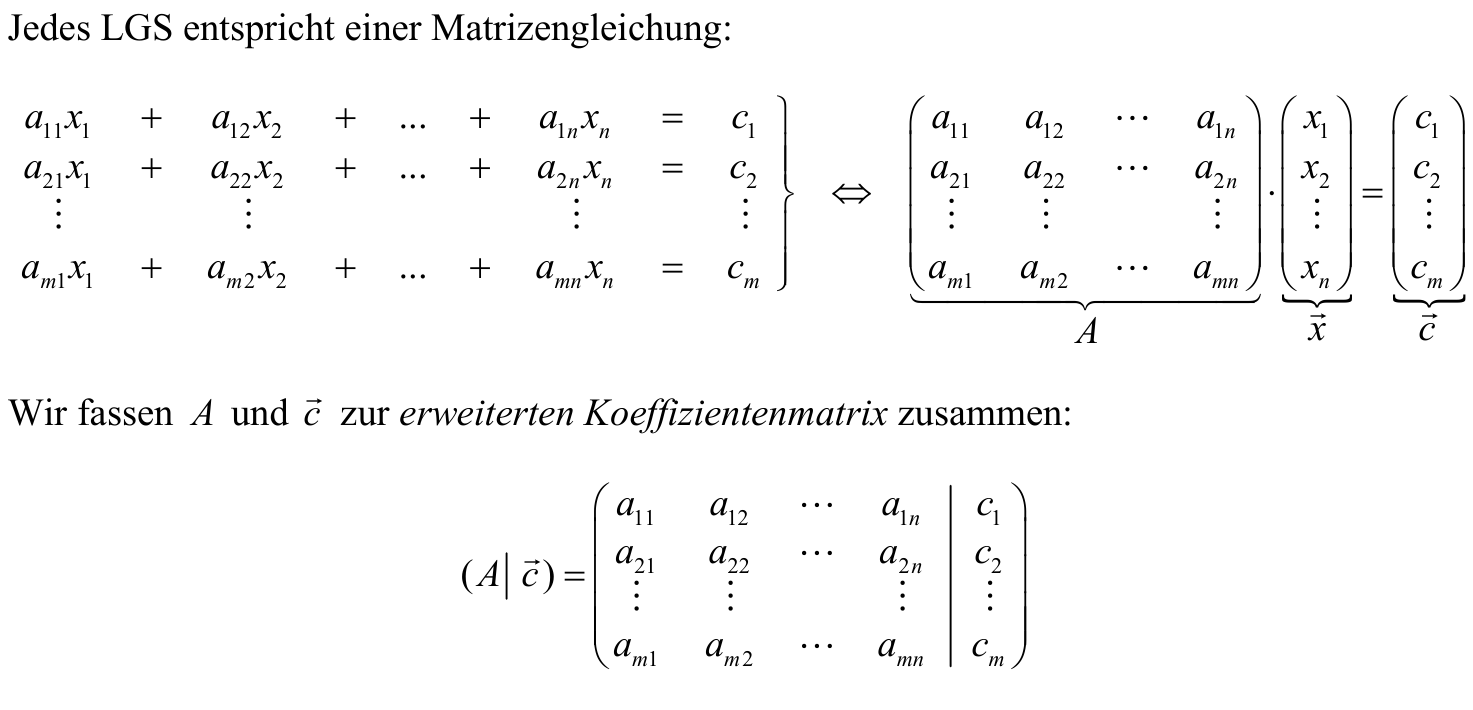
\includegraphics[width=\linewidth]{img/lgs.png}
\end{figure}
\subsection{Zeilenstufenformen}
Die Zeilenstufenform wird durch gewichtete Additionen erreicht, mit welchen gewisse Koeffizienten eliminiert werden können. Unter einem Zeilenführer versteht man das erste Element einer Zeile, das nicht 0 ist. Die Zeilenstufenform ist erreicht, wenn jeder Zeilenführer eine 1 ist und jeder Zeilenführer weiter rechts vom darüber liegenden Zeilfenführer liegt und Nullzeilen ganz unten sind. Die \textbf{reduzierte Zeilenstufenform} wird erreicht, indem von der normalen Zeilenstufenform ausgehend alle Spaltenelemente in der sich ein Zeilenführer befindet mit gewichteten Additionen auf 0 gesetzt werden.

\subsection{Gauss-Jordan-Algorithmus}
Der Gauss-Jordan-Algorithmus wird angewendet um eine Koeffizientenmatrix in die reduzierte Zeilenstufenform zu bringen. Der Algorithmus verwendet wiederholte, gewichtete Additionen und Matrixoperationen um die reduzierte Zeilenstufenform zu erreichen.

\end{document}
